\documentclass[11pt]{beamer}

\usetheme{metropolis}

\usepackage{graphicx}
\usepackage{physics}
\usepackage{adjustbox}
\usepackage{caption}
\usepackage{chemformula}
\usepackage{quoting}
\usepackage[style=chem-angew,backend=bibtex]{biblatex}
\bibliography{references}
%
% Choose how your presentation looks.
%
% For more themes, color themes and font themes, see:
% http://deic.uab.es/~iblanes/beamer_gallery/index_by_theme.html
%
\mode<presentation>
{
  \usetheme{default}      % or try Darmstadt, Madrid, Warsaw, ...
  \usecolortheme{default} % or try albatross, beaver, crane, ...
  \usefonttheme{default}  % or try serif, structurebold, ...
  \setbeamertemplate{navigation symbols}{}
  \setbeamertemplate{caption}[numbered]
  \setbeamerfont{footnote}{size=\tiny}
} 

\usepackage[english]{babel}
\usepackage[utf8]{inputenc}
\graphicspath{{image/}}

\AtBeginSection[]{
\begin{frame}{Outline}
  \tableofcontents[currentsection]
\end{frame}
}

\title{Chapter 1: Sharpening the Math Toolbox}
\institute{Chemistry Department, Cypress College}
\date{August 23, 2022}

\begin{document}

\begin{frame}
  \titlepage
\end{frame}

\section{Introduction: Who Am I?}

\begin{frame}{Introduction: Who am I?}
  \begin{center}
    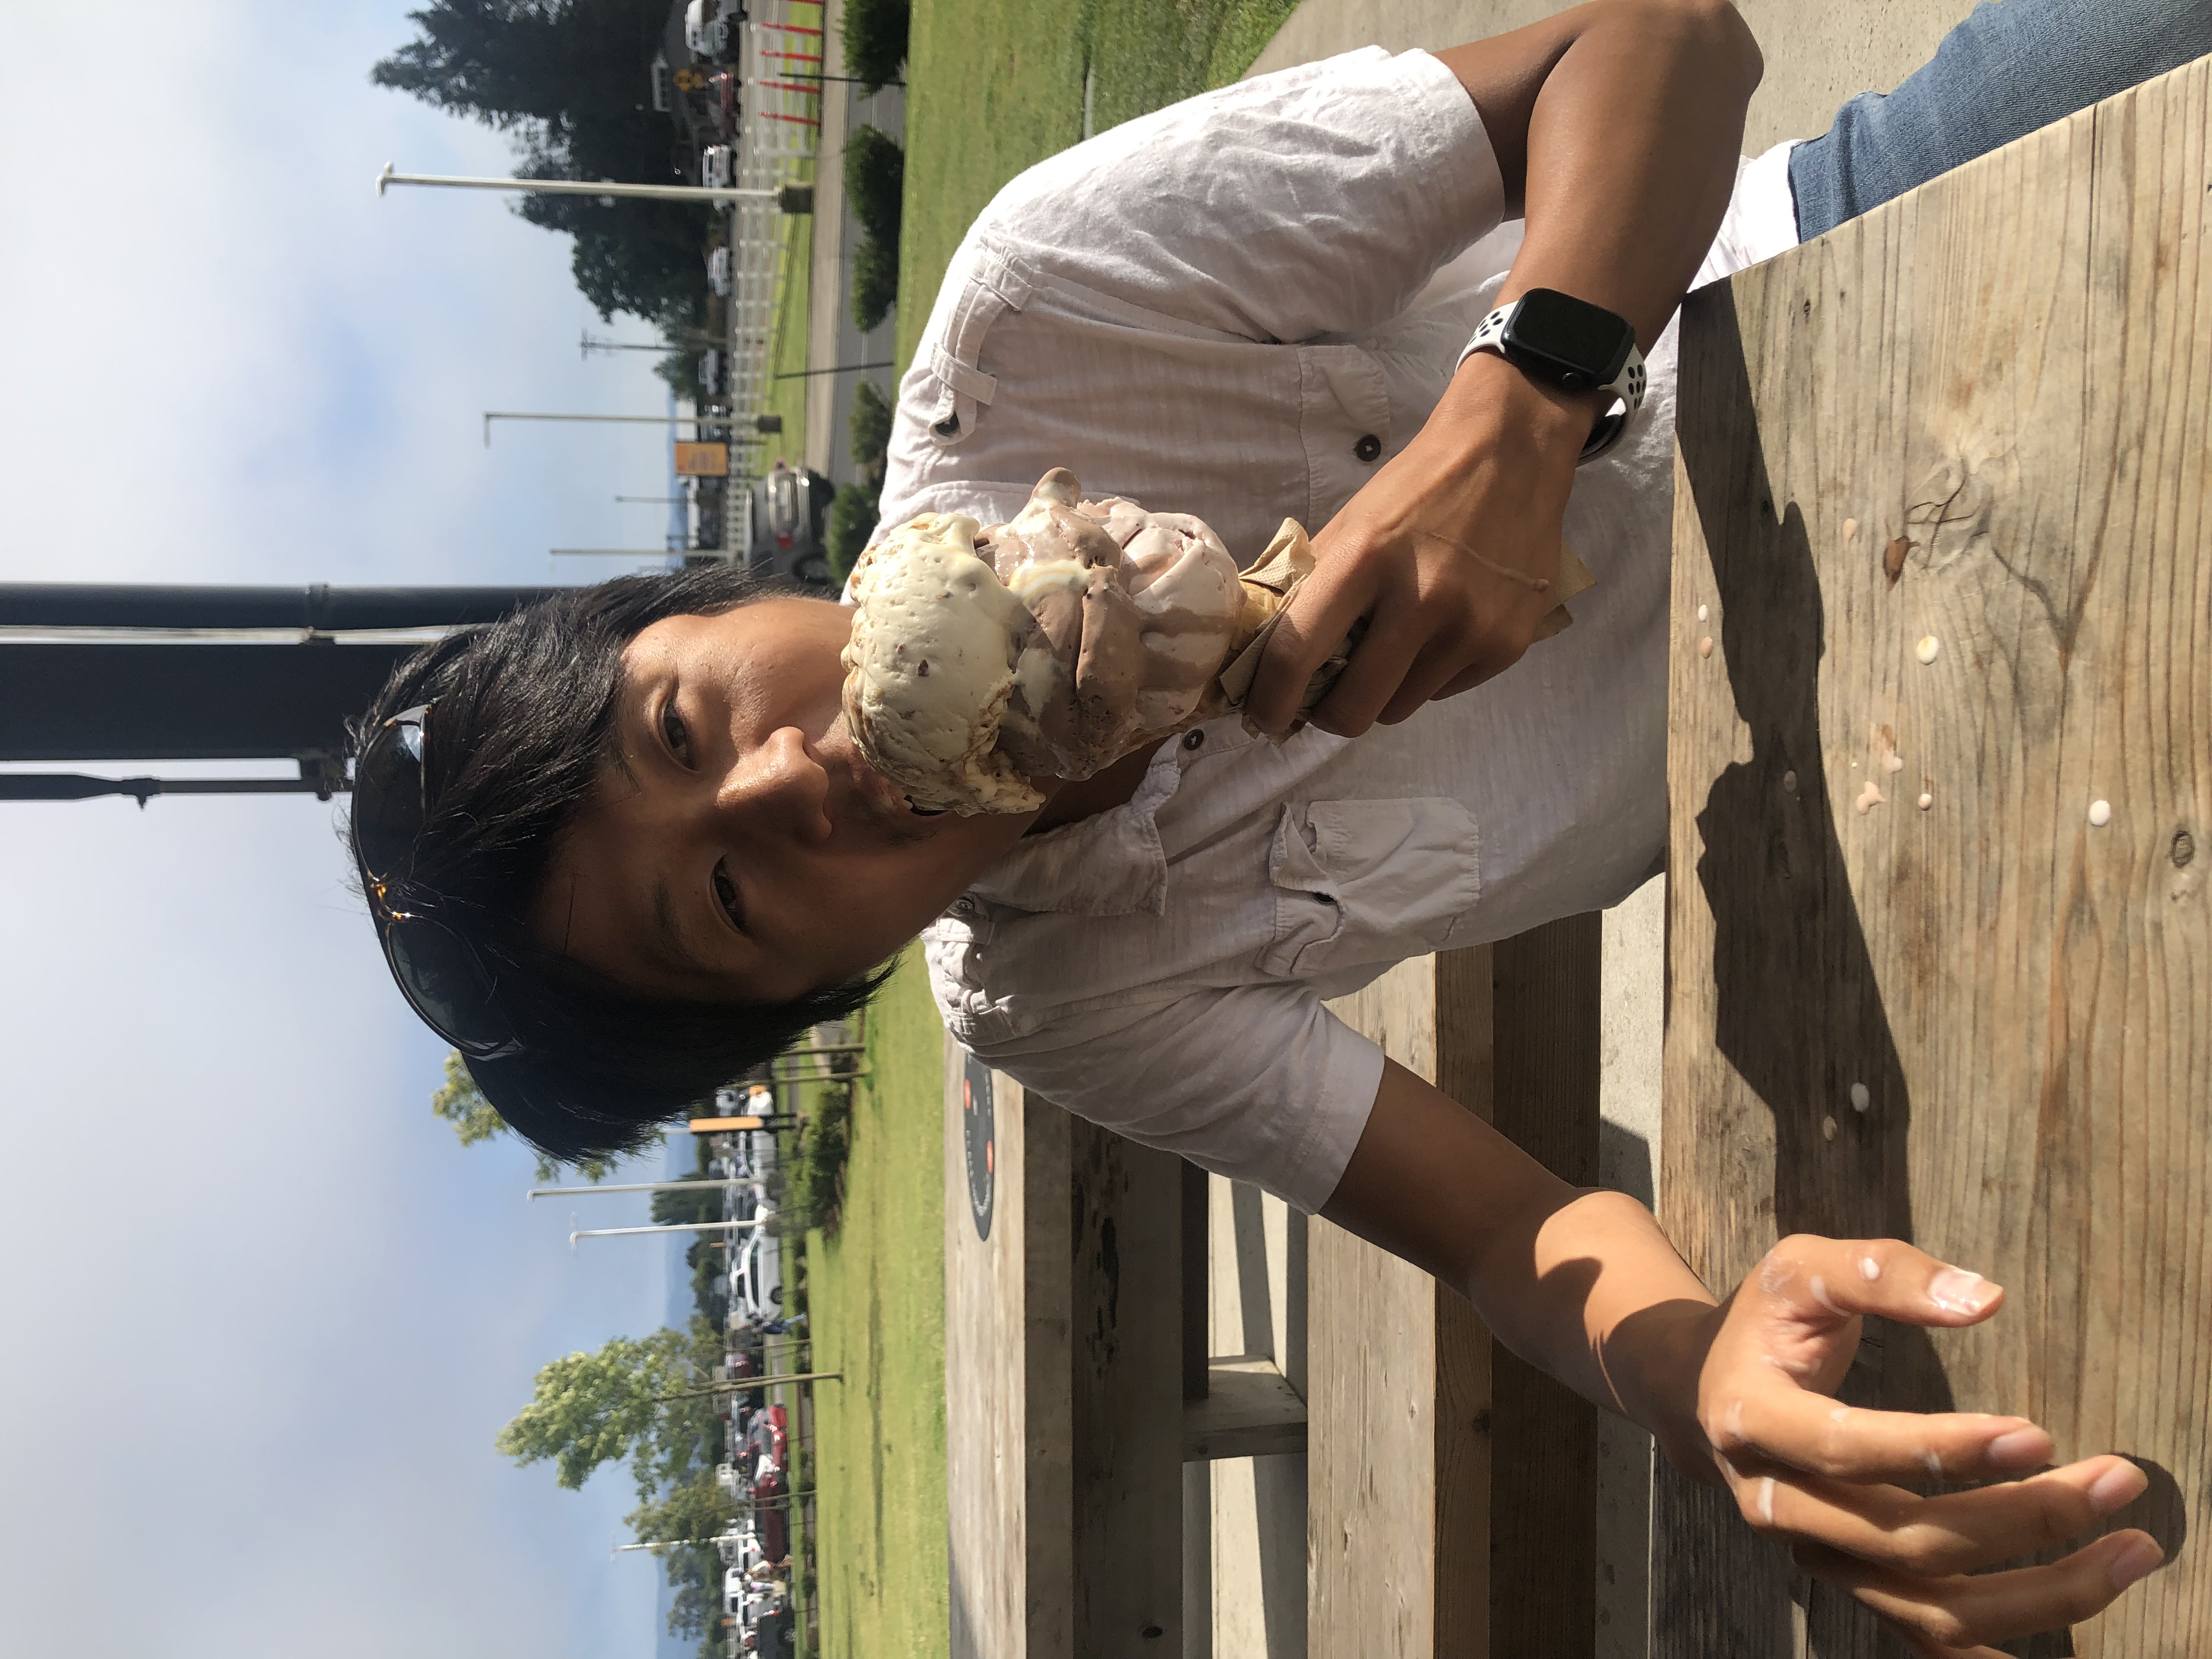
\includegraphics[angle=-90,origin=c,scale=0.03]{triple_ice}
  \end{center}
  \begin{itemize}
  \item Last June, graduated from University of California, Irvine,
    receiving my PhD in Computational and Theoretical Chemistry
  \item May refer me as Dr. Prof. Brian D. Nguyen
  \item Exercising, driving, hiking, learning new languages, and gaming
  \end{itemize}
\end{frame}

\begin{frame}{Teaching Philosophy}
  \textbf{Humanist-inspired pedagogy:}
  \begin{itemize}
  \item Student-teacher relationship is central
    \begin{itemize}
    \item Mutual respect and growth
    \item ``Unconditional positive regard''
    \item Awareness of the other and their thoughts/emotions
    \item Teacher is coach/supporter/mentor rather than supervisor/boss
    \end{itemize}
  \item Focus on attitude and approach rather than content
  \item Learning to fail
  \item Collaboration rather than competition
  \item Explore and experience something new together, learn about
    chemistry and ourselves
  \end{itemize}
\end{frame}

\begin{frame}{Making the Most of It}

  Questions to consider:
  \begin{itemize}
  \item Why am I taking this course?
  \item What would I like to achieve?
  \item What methods/tools/resources work for me?
  \end{itemize}

  Your feedback, questions, participation are vital:
  \begin{itemize}
  \item Attend lectures and discussions, if possible
  \item Give on-going feedback to instructors through facial expression,
    emojis, chat, email, during office hours etc.
  \item Fill out evaluations
  \item Own your education
  \item Be proactive, do not hesitate to speak up or get help
  \end{itemize}

\end{frame}

\begin{frame}{Introduction: Your Turn}
  \textbf{With your notecard:}
  \begin{itemize}
  \item Take 2-3 mins and write down your name on one side
  \item On the other side, write down something that I can
    remember you by
  \end{itemize}
\end{frame}

\section{Review: Syllabus}

\section{Math Review for Chemist}

\begin{frame}
  \vspace{1in}
  \begin{quote}
    Chemistry is necessarily an experimental science: its
    conclusions are drawn from data, and its principles
    supported by evidence from facts. - Michael Faraday
  \end{quote}
  
  \begin{center}
    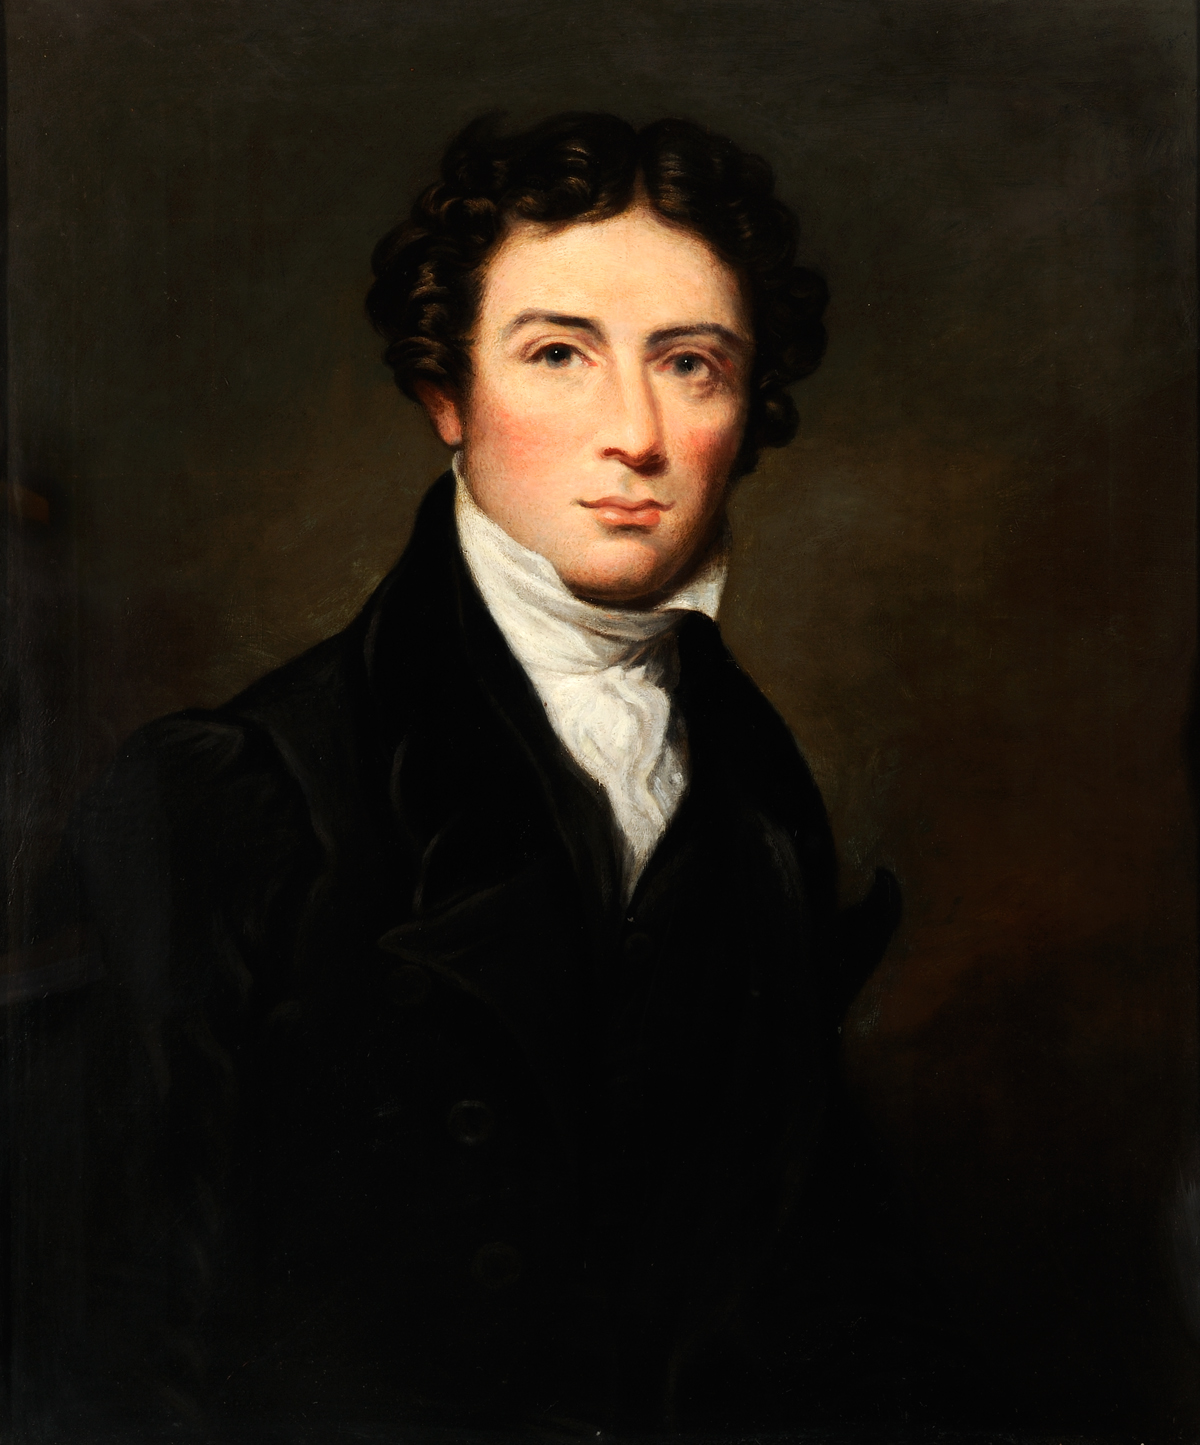
\includegraphics[scale=0.08]{micahel_fara}
  \end{center}
\end{frame}

\begin{frame}{Scientific Notation}
  Often with large numbers, the scientific notation is
  needed and expressed by
  \begin{equation}
    N = C \times 10^m
  \end{equation}
  where $N$ is a large number, $C$ is the coefficient (a number between $1-9$)
  and $m$ is the exponent (a positive or negative integer)

  \textbf{Example:} $0.00363246 = 3.63246 \times 10^{-3}$

\end{frame}

\begin{frame}{Significant Figures}
  \begin{itemize}
  \item The meaningful digits in a measured or calculated
    quantity
  \item Example: $0.00363246 \simeq 3.63 \times 10^{-3}$ to three
    sig figures
  \item Implies relative accuracy of $10^{-m}$, e.g. $0.1\%$ for $m=3$
  \item[] \begin{center}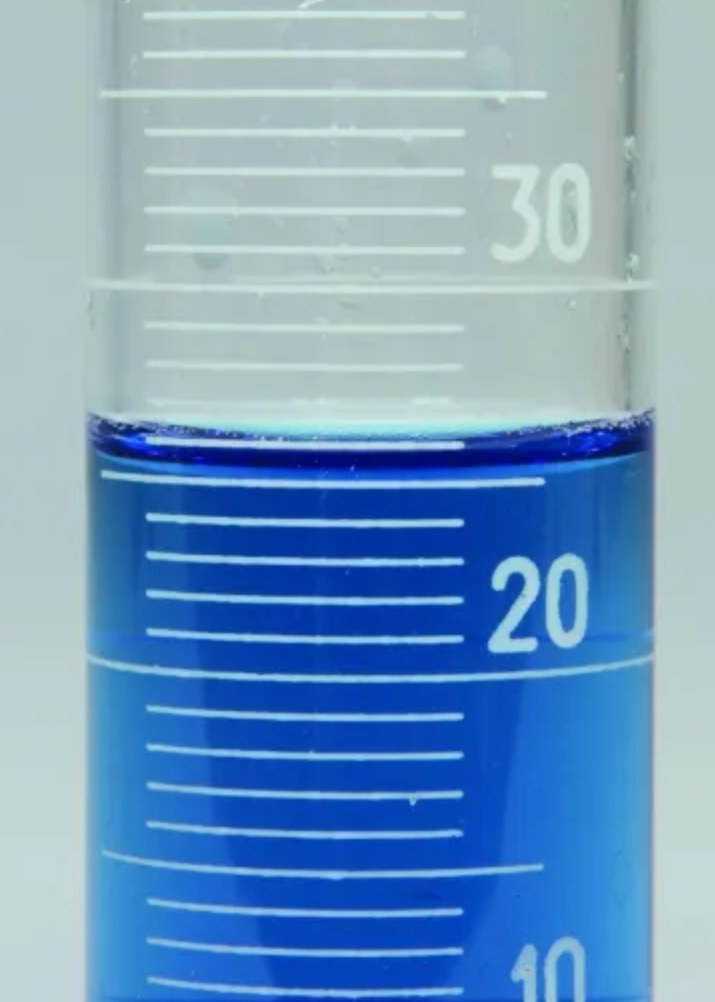
\includegraphics[scale=0.1]{grad}
  \end{center}
  \item For practice, what is the measured volume for the liquid
    above?
  \end{itemize}
\end{frame}

\begin{frame}{Significant Figures - More Practice!}
  \centering
  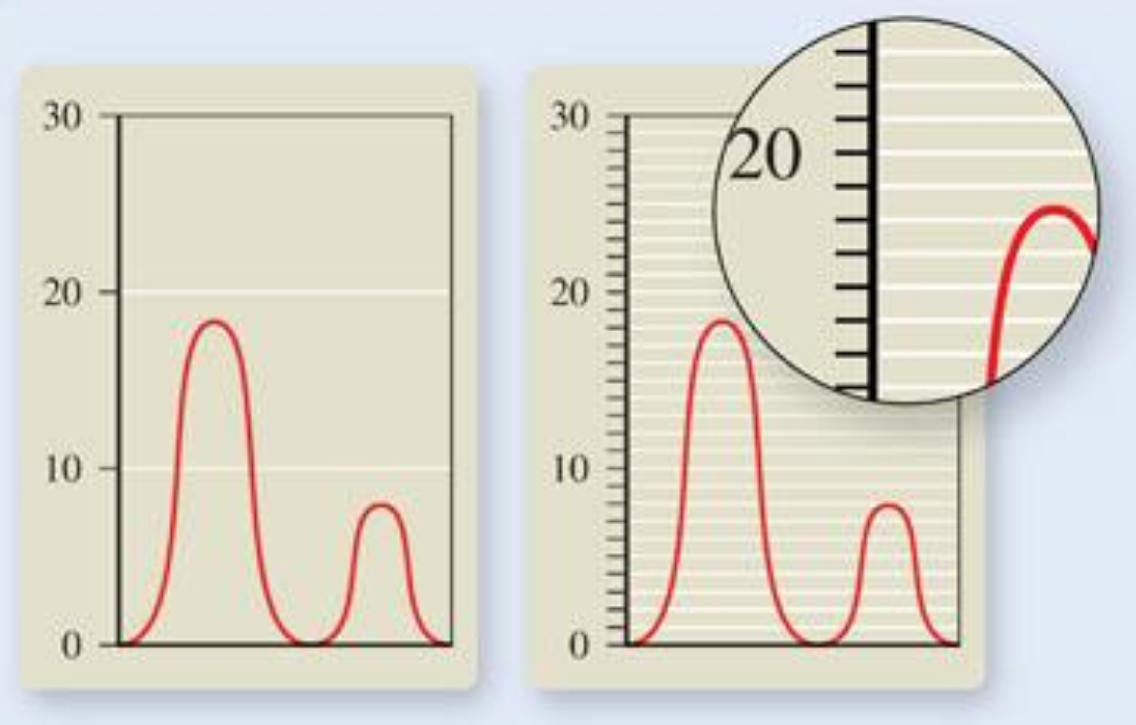
\includegraphics[scale=0.22]{graph_measure}

  \textbf{Which is relatively more accurate? What is the
    approximate measurement for each graph? What is missing?}
\end{frame}

\begin{frame}{Counting Significant Figures}
  All \textbf{non-zero} numbers in a measured number are
  significant

  \textbf{Practice:} What is the number of significant figures?
  \begin{itemize}
  \item 36.1 ft
  \item 1 dozen eggs
  \item 155.6 lbs
  \end{itemize}
\end{frame}

\begin{frame}{Leading, Sandwiched and Trailing Zeroes}
  \textbf{Leading zeroes:} Precede non-zero digits in a
  decimal number are \textbf{not} significant

  \textbf{Sandwiched zeroes:} Occur between nonzero numbers are significant
  
  \textbf{Trailing zeroes:} Following non-zero numbers are
  significant in numbers with a decimal point
\end{frame}

\begin{frame}{Leading, Sandwiched and Trailing Zeroes}
  \textbf{Practice:} What is the number of significant figures?
  \begin{itemize}
  \item 0.0702 lb
  \item 48600 L
  \item 100.000 g
  \item 1.020 atm
  \item $9.01 \times 10^5$ m
  \end{itemize}
\end{frame}

\begin{frame}{Calculated Answers}
  \centering
  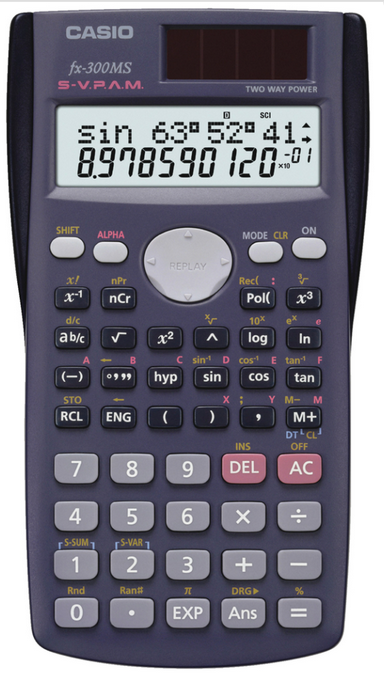
\includegraphics[scale=0.2]{calc}
  \begin{itemize}
  \item Answers must have the same number of significant
    figures as the least precise measured number(s)
  \item Calculator answers must often be \textbf{rounded off}
  \item \textbf{Rounding rules} are used to obtain the correct
    number of significant figures
  \end{itemize}
\end{frame}

\begin{frame}{\textbf{Practice:} Round to four significant figures.}
  \begin{itemize}
  \item 824.75143 cm
  \item 0.112544 g
  \end{itemize}
\end{frame}

\begin{frame}{Calculation: Rules for Rounding}
  \textbf{Rule 1:} In carrying out a multiplication or division,
  the answer cannot have more significant figures than either of
  the original numbers.

  \textbf{Example:}
  \begin{equation}
    \frac{278 \text{mi}}{11.70 \text{gal}} = 23.8 \text{mi/gal}
  \end{equation}
  
\end{frame}

\begin{frame}{Calculation: Rules for Rounding}
  \textbf{Rule 2:} In carrying out an addition or subtraction, the
  answer cannot have more digits after the decimal point than either
  of the original numbers or more digits after the leftmost uncertain
  digit than either of the original numbers.

  \textbf{Example:}
  \begin{equation}
    3.18 \text{L} + 0.01315 \text{L} = 3.19 \text{L}
  \end{equation}
\end{frame}

\begin{frame}{TIPS: Avoid Rounding Errors}
  \begin{itemize}
  \item Carry at least 2 extra significant figures in
    intermediate results!
  \item You will need to report your results \emph{exactly} to a
    given precision
  \item Round at the very end
  \end{itemize}

\end{frame}

\begin{frame}{Accuracy vs. Precision}
  \textbf{What is the difference between accuracy
    and precision?}

  \centering
  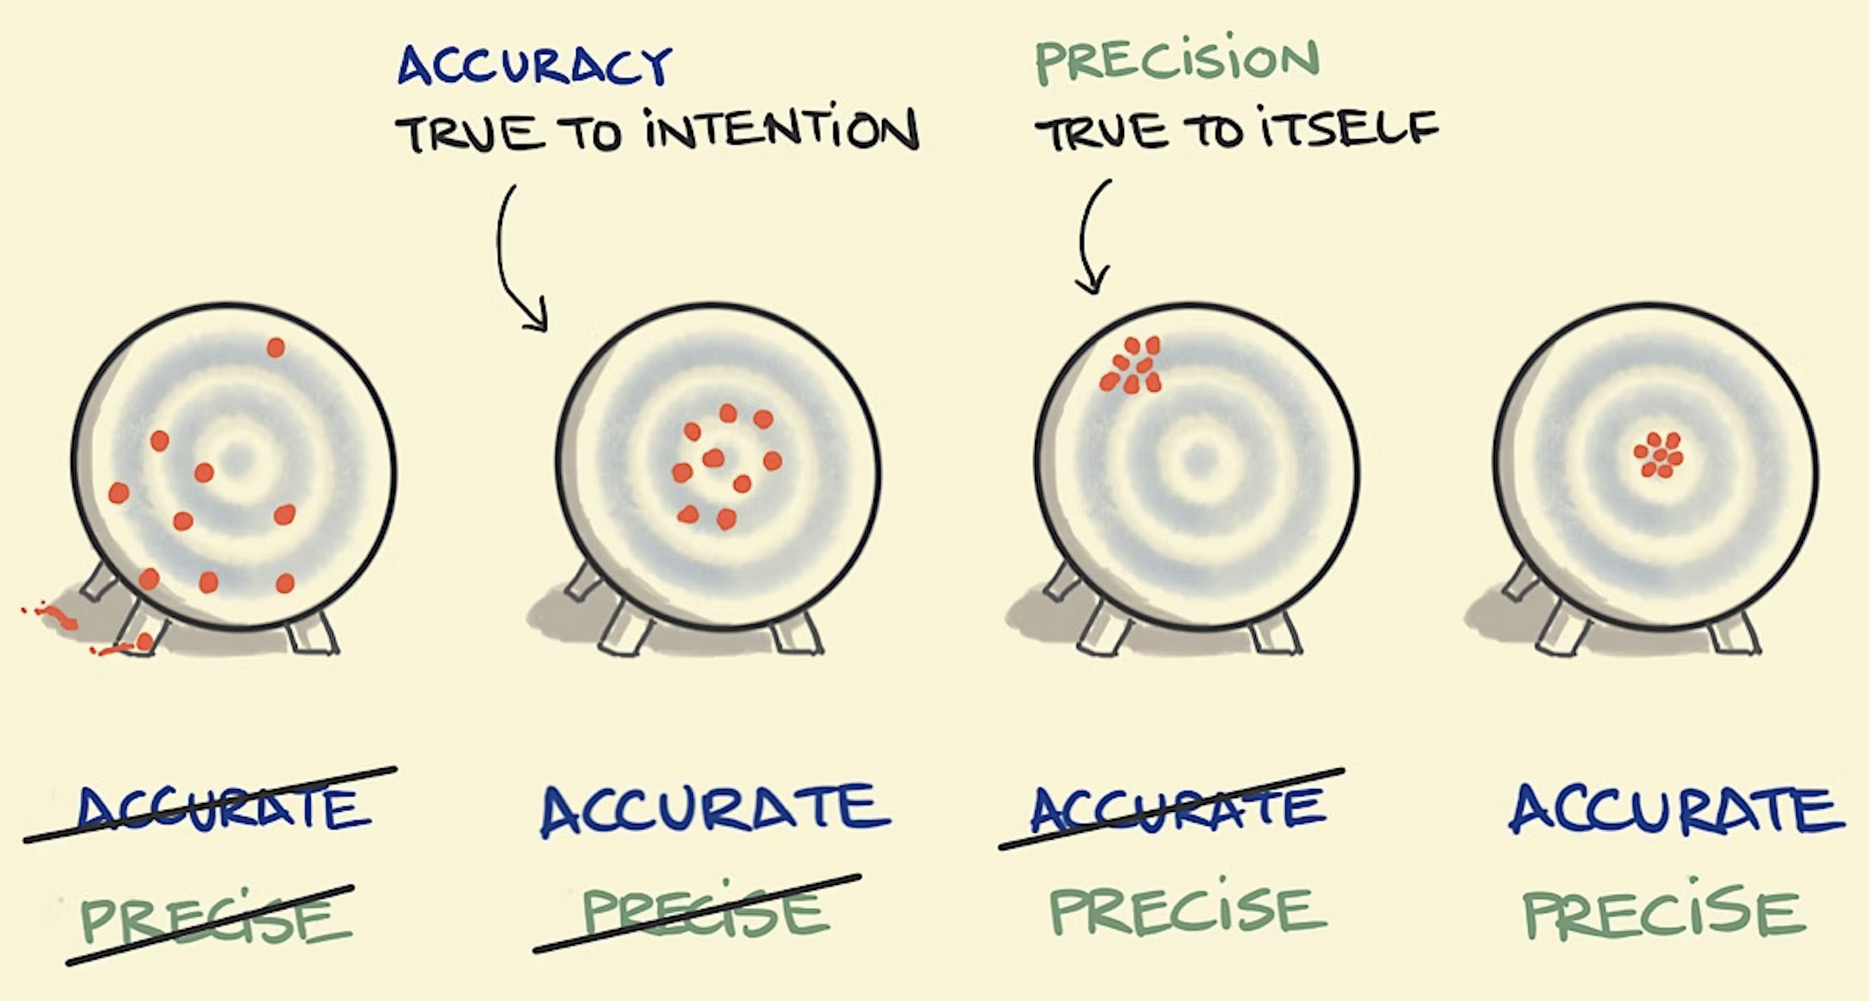
\includegraphics[scale=0.15]{accur_prec.png}
\end{frame}

\begin{frame}{Accuracy vs. Precision}
  \textbf{Accuracy}
  \begin{itemize}
  \item How close you are to the actual value
  \item Calculated by the forumula
  \item[] \begin{equation}
    \% \text{Error} = \frac{\text{measured} - \text{actual}}{\text{actual}}
  \end{equation}
  \end{itemize}
  
  \textbf{Precision}
  \begin{itemize}
  \item How finely tuned your measurements are or
    how close they can be to each other
  \item Depends on the measuring tool
  \item Implied by the number of significant figures
  \end{itemize}
\end{frame}

\begin{frame}{Importance of Units}
  \centering
  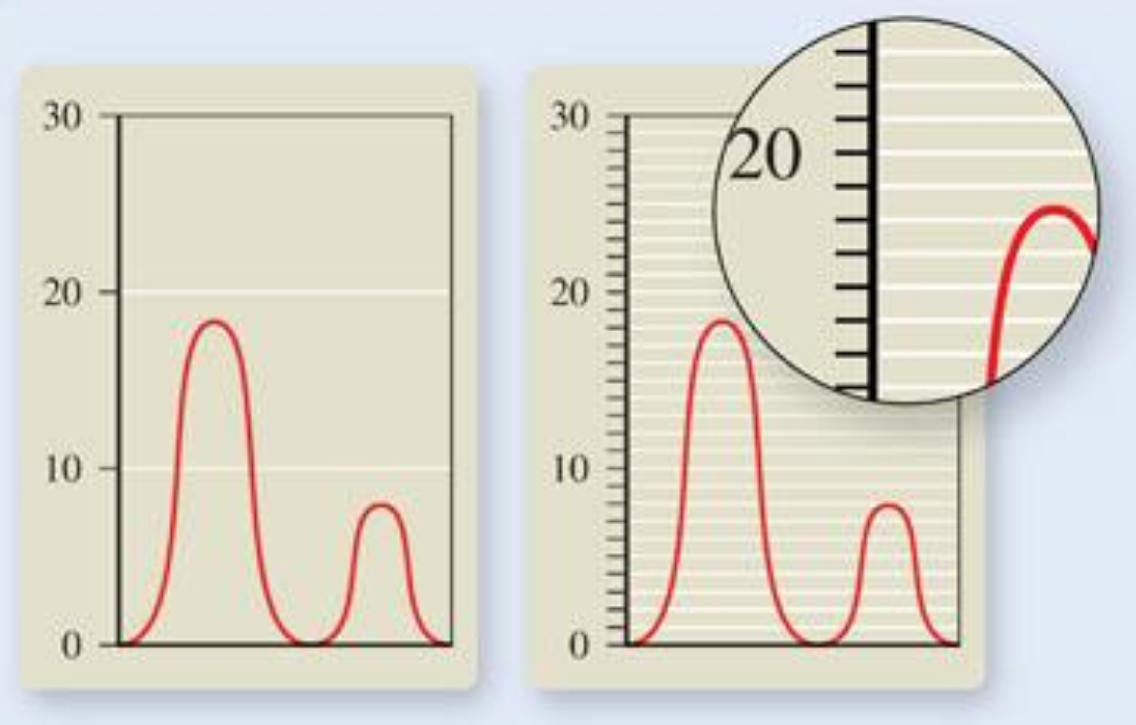
\includegraphics[scale=0.15]{graph_measure}

  \begin{itemize}
  \item Numbers with no units have \textbf{no}
    meaning
  \item As scientists, we look at the following
  \end{itemize}
  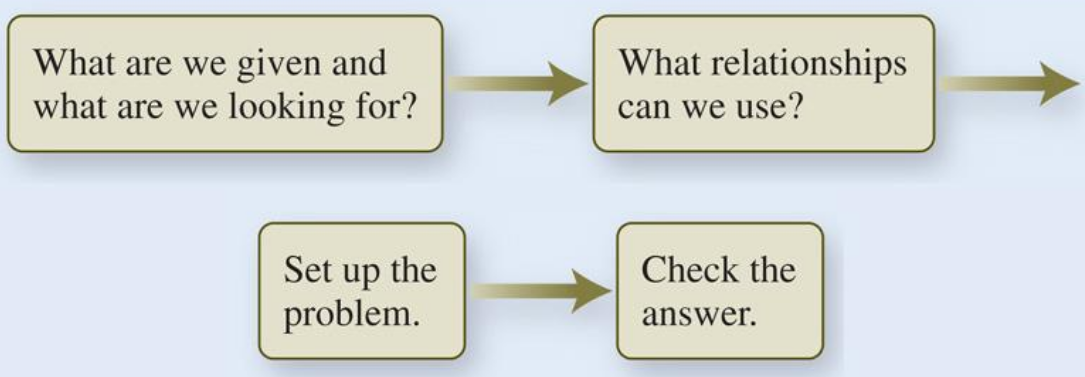
\includegraphics[scale=0.2]{unit_qs}
\end{frame}

\begin{frame}{Prefixes of Metric System}
  \centering
  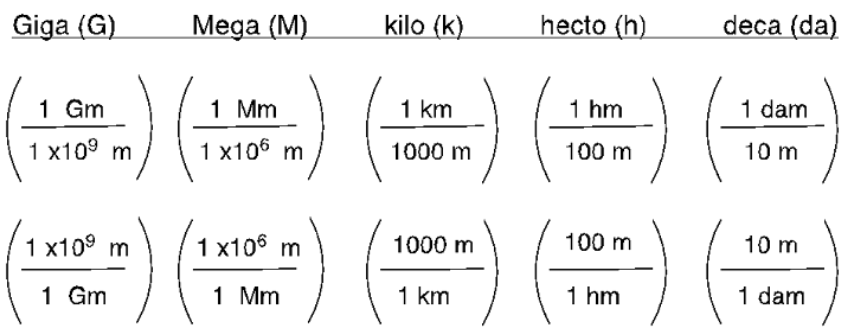
\includegraphics[scale=0.3]{metric_1}
  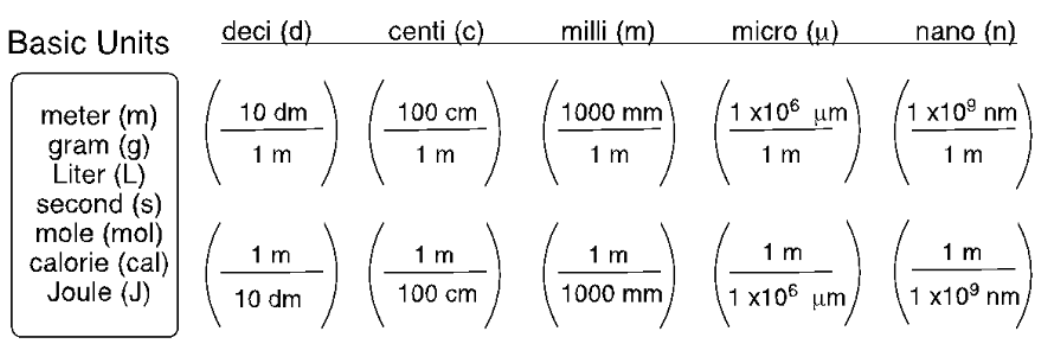
\includegraphics[scale=0.3]{metric_2}
\end{frame}

\begin{frame}{Unit Conversion}
  \textbf{Dimensional Analysis:} A quantity in one unit is converted
  to an equivalent quantity in a different unit by using conversion
  factors that express the relationship between units.

  \begin{equation}
    (\text{Starting quantity})\times (\text{Conversion factor})
    = \text{Equivalent quantity}
  \end{equation}

  \textbf{Examples:}
  \begin{itemize}
  \item 1 min = 60 secs
  \item 1 lb = 16 oz
  \item 2.20 lb = 1 kg
  \item 2.54 cm = 1 in
  \end{itemize}
\end{frame}

\begin{frame}{Relating Mass and Volume}
  \begin{itemize}
  \item Density ($D$) is a convenient means of obtaining the
    mass ($M$) from its volume ($V$) or vice versa
  \item[] \begin{equation}
    D = M/V
  \end{equation}
  \end{itemize}
\end{frame}

\begin{frame}{Strategy for Dimensional Analysis}
  \begin{enumerate}
  \item Identify the information given and the
    information needed to answer.
  \item Find the relationship(s) between the known
    information and unknown answer, and plan a series
    of steps, including conversion factors, for getting from
    one to the other.
  \item Solve the problem by canceling units.
  \item Check the answer to make sure it makes sense,
    both in magnitude and units.
  \end{enumerate}
\end{frame}

\begin{frame}{Whiteboard: Dimensional Analysis}
\end{frame}

\end{document}
